\section{联邦学习数据集}
\addcontentsline{toe}{section}{{5.2\ \ Datasets for Federated Learning}\numberline\,}
\label{sec:chap5-datasets}

% NOT finished
% NOT indexed

正如\S\ref{sec:chap1-fl-applications}~中提到的,联邦学习所涉及、处理的实际数据往往具有强烈的统计异质性,因此我们用于仿真试验的试验数据集需要以多种方式、从多个角度尽量模拟、贴近这种统计异质性。比较幸运的是,在本章\S\ref{sec:chap5-design}中提到的一些联邦学习算法框架,尤其是

\begin{table}[htbp]
\centering
\begin{threeparttable}[b]
\begin{tabular}{|c|c|c|c|c|}
\hlineB{3.5}
数据集名称 & 规模 & 默认节点数目 & 任务 & 样本类型 \\
\hline \hline
MNIST\tnote{$\ast$} & 60000 & 1000 & 图像分类 & $28\times 28$的单通道灰度图像 \\
EMNIST\tnote{$\ast$} & 749068 & 3400 & 图像分类 & $28\times 28$的单通道灰度图像 \\
CIFAR10/100 & 60000 & 500 & 图像分类 & $32\times 32$的RGB3通道图像 \\
Shakespeare & 18424 & 715 & 下一字符预测 & 文本 \\
Sent140 & 40783 & 715 & 文本情感分类 & 文本 \\
Synthetic($\alpha, \beta$)\tnote{$\ast\ast$} & N/A & N/A & 分类 & 随机生成的高维向量 \\
\hlineB{3.5}
\end{tabular}
\begin{tablenotes}
\item[$\ast$] {\smaller 这两个数据集还有经过筛选\cite{sahu2018fedprox}的规模更小的数据子集,也被本文实现的联邦学习仿真系统所包含。}
\item[$\ast\ast$] {\smaller 参数$\alpha, \beta$是两个独立的均值为$0$的正态分布的标准差,用于模拟节点内以及节点间的数据分布差异。}
\end{tablenotes}
\caption{本文开发的联邦学习仿真系统内置的数据集}
\label{tab:datasets}
\end{threeparttable}
\end{table}


\begin{figure}[H]
\centering
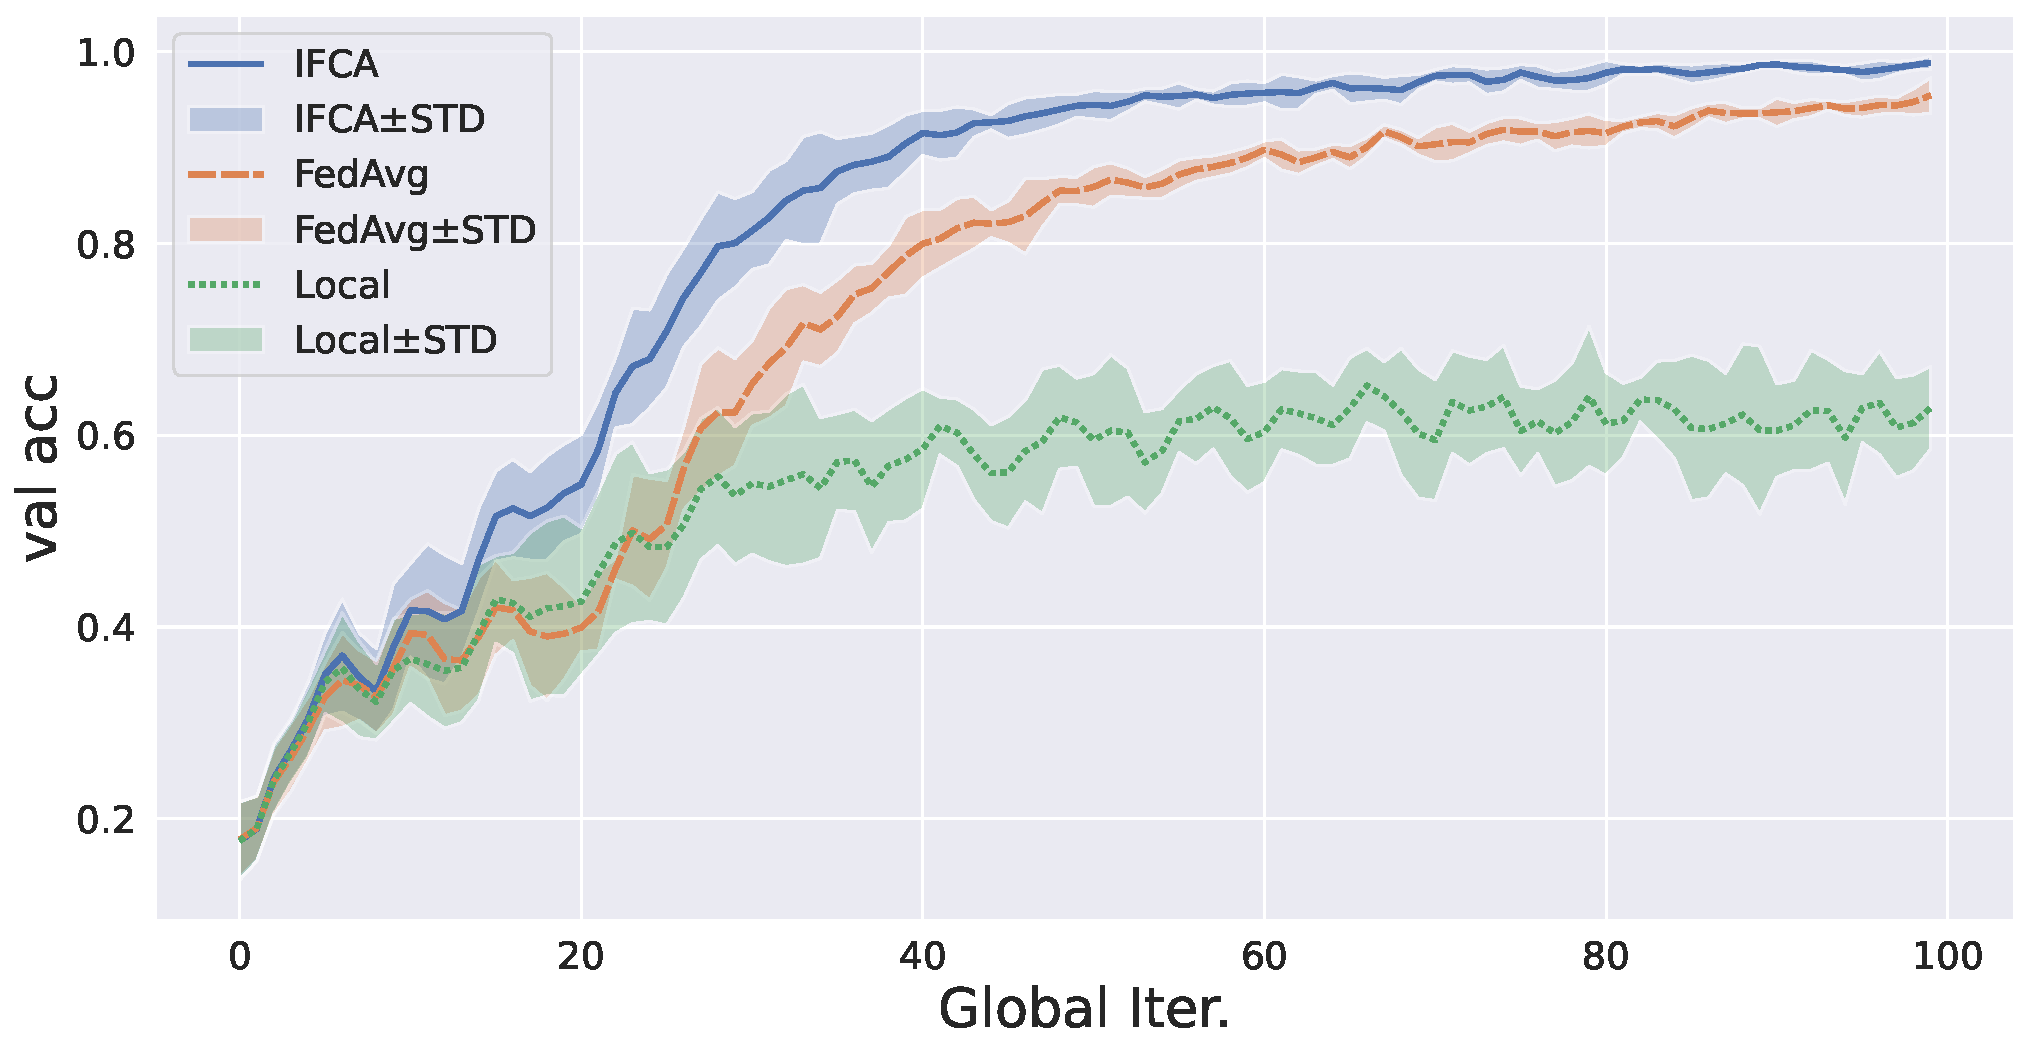
\includegraphics[width=\textwidth]{figures/fedproxfemnist.pdf}
\caption{待写}
\label{fig:fedproxfemnist-experiment}
\end{figure}

待写。。。。
